\begin{figure}[H]
\centering


\tikzset{every picture/.style={line width=0.75pt}} %set default line width to 0.75pt        

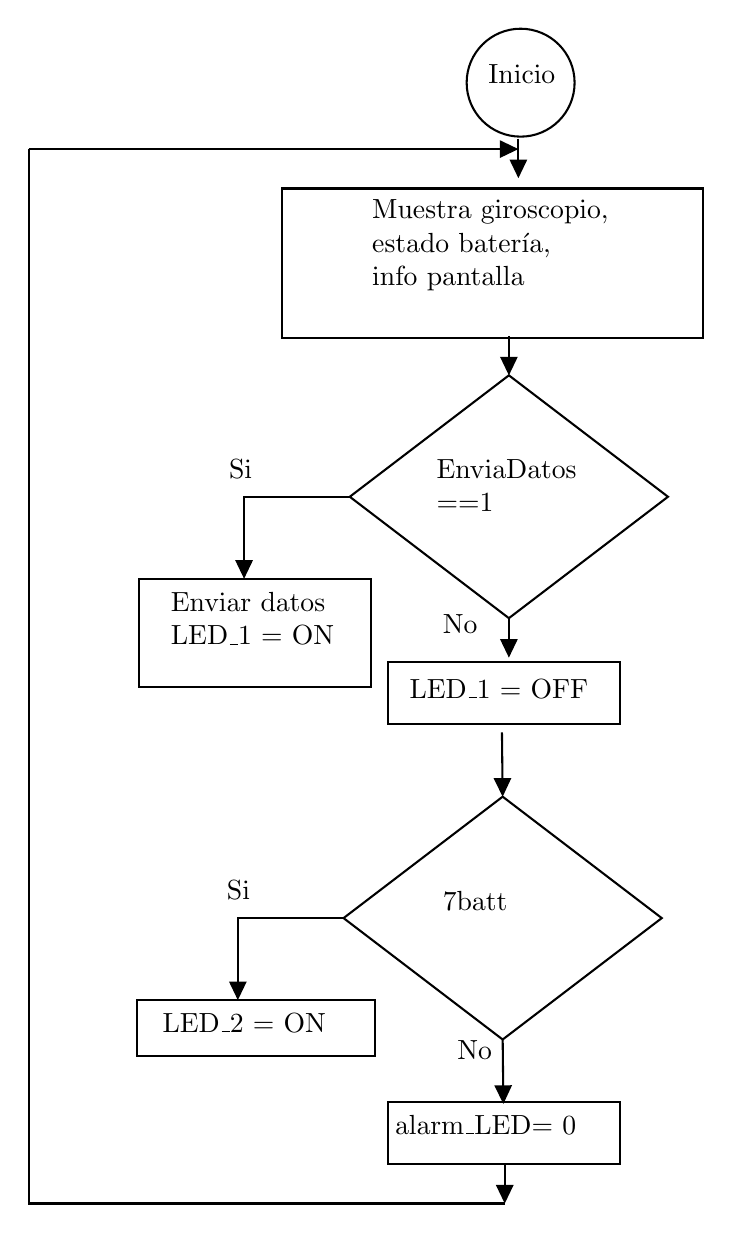
\begin{tikzpicture}[x=0.75pt,y=0.75pt,yscale=-1,xscale=1]
%uncomment if require: \path (0,616); %set diagram left start at 0, and has height of 616

%Flowchart: Connector [id:dp7813495520702245] 
\draw   (315,40) .. controls (315,25.64) and (326.64,14) .. (341,14) .. controls (355.36,14) and (367,25.64) .. (367,40) .. controls (367,54.36) and (355.36,66) .. (341,66) .. controls (326.64,66) and (315,54.36) .. (315,40) -- cycle ;
%Straight Lines [id:da8847526091998554] 
\draw    (339.92,67) -- (339.92,83) ;
\draw [shift={(339.92,86)}, rotate = 270] [fill={rgb, 255:red, 0; green, 0; blue, 0 }  ][line width=0.08]  [draw opacity=0] (8.93,-4.29) -- (0,0) -- (8.93,4.29) -- cycle    ;
%Flowchart: Decision [id:dp21596588394867888] 
\draw   (335.35,181) -- (412,239.5) -- (335.35,298) -- (258.69,239.5) -- cycle ;
%Straight Lines [id:da7204417446380422] 
\draw    (335.35,162) -- (335.35,178) ;
\draw [shift={(335.35,181)}, rotate = 270] [fill={rgb, 255:red, 0; green, 0; blue, 0 }  ][line width=0.08]  [draw opacity=0] (8.93,-4.29) -- (0,0) -- (8.93,4.29) -- cycle    ;
%Straight Lines [id:da49582350632228556] 
\draw    (207.76,260) -- (207.76,276) ;
\draw [shift={(207.76,279)}, rotate = 270] [fill={rgb, 255:red, 0; green, 0; blue, 0 }  ][line width=0.08]  [draw opacity=0] (8.93,-4.29) -- (0,0) -- (8.93,4.29) -- cycle    ;
%Shape: Right Angle [id:dp2914826540765745] 
\draw   (258.69,239.5) -- (207.76,239.5) -- (207.76,260) ;
%Shape: Right Angle [id:dp7943090498770735] 
\draw   (333.35,580) -- (104,580) -- (104,72) ;
%Straight Lines [id:da15691850789793538] 
\draw    (332,353) -- (332.31,381) ;
\draw [shift={(332.35,384)}, rotate = 269.36] [fill={rgb, 255:red, 0; green, 0; blue, 0 }  ][line width=0.08]  [draw opacity=0] (8.93,-4.29) -- (0,0) -- (8.93,4.29) -- cycle    ;
%Flowchart: Process [id:dp025828036440153967] 
\draw   (157,279) -- (269,279) -- (269,331) -- (157,331) -- cycle ;
%Flowchart: Process [id:dp08317044111396199] 
\draw   (226,91) -- (429,91) -- (429,163) -- (226,163) -- cycle ;
%Flowchart: Decision [id:dp9588588712187942] 
\draw   (332.35,384) -- (409,442.5) -- (332.35,501) -- (255.69,442.5) -- cycle ;
%Straight Lines [id:da6075623967992321] 
\draw    (335.35,298) -- (335.35,314) ;
\draw [shift={(335.35,317)}, rotate = 270] [fill={rgb, 255:red, 0; green, 0; blue, 0 }  ][line width=0.08]  [draw opacity=0] (8.93,-4.29) -- (0,0) -- (8.93,4.29) -- cycle    ;
%Straight Lines [id:da7280821078053175] 
\draw    (204.76,463) -- (204.76,479) ;
\draw [shift={(204.76,482)}, rotate = 270] [fill={rgb, 255:red, 0; green, 0; blue, 0 }  ][line width=0.08]  [draw opacity=0] (8.93,-4.29) -- (0,0) -- (8.93,4.29) -- cycle    ;
%Shape: Right Angle [id:dp5301940302382446] 
\draw   (255.69,442.5) -- (204.76,442.5) -- (204.76,463) ;
%Flowchart: Process [id:dp03155186296961898] 
\draw   (156,482) -- (271,482) -- (271,509) -- (156,509) -- cycle ;
%Straight Lines [id:da1967066179049608] 
\draw    (333.35,561) -- (333.35,577) ;
\draw [shift={(333.35,580)}, rotate = 270] [fill={rgb, 255:red, 0; green, 0; blue, 0 }  ][line width=0.08]  [draw opacity=0] (8.93,-4.29) -- (0,0) -- (8.93,4.29) -- cycle    ;
%Flowchart: Process [id:dp5138152311739683] 
\draw   (277,319) -- (389,319) -- (389,349) -- (277,349) -- cycle ;
%Flowchart: Process [id:dp3581810005977748] 
\draw   (277,531) -- (389,531) -- (389,561) -- (277,561) -- cycle ;
%Straight Lines [id:da864404406808954] 
\draw    (332.35,501) -- (332.66,529) ;
\draw [shift={(332.69,532)}, rotate = 269.36] [fill={rgb, 255:red, 0; green, 0; blue, 0 }  ][line width=0.08]  [draw opacity=0] (8.93,-4.29) -- (0,0) -- (8.93,4.29) -- cycle    ;
%Straight Lines [id:da9757080202876469] 
\draw    (104,72) -- (336.92,72) ;
\draw [shift={(339.92,72)}, rotate = 180] [fill={rgb, 255:red, 0; green, 0; blue, 0 }  ][line width=0.08]  [draw opacity=0] (8.93,-4.29) -- (0,0) -- (8.93,4.29) -- cycle    ;

% Text Node
\draw (324,30) node [anchor=north west][inner sep=0.75pt]   [align=left] {Inicio};
% Text Node
\draw (299,220) node [anchor=north west][inner sep=0.75pt]   [align=left] {EnviaDatos\\==1};
% Text Node
\draw (302,295) node [anchor=north west][inner sep=0.75pt]   [align=left] {No};
% Text Node
\draw (199,220) node [anchor=north west][inner sep=0.75pt]   [align=left] {Si};
% Text Node
\draw (171,284) node [anchor=north west][inner sep=0.75pt]   [align=left] {Enviar datos\\LED\_1 = ON};
% Text Node
\draw (268,95) node [anchor=north west][inner sep=0.75pt]   [align=left] {Muestra giroscopio,\\estado batería,\\info pantalla};
% Text Node
\draw (302,428) node [anchor=north west][inner sep=0.75pt]   [align=left] {$\displaystyle 7\geqslant $batt};
% Text Node
\draw (198,423) node [anchor=north west][inner sep=0.75pt]   [align=left] {Si};
% Text Node
\draw (167,487) node [anchor=north west][inner sep=0.75pt]   [align=left] {LED\_2 = ON};
% Text Node
\draw (309,500) node [anchor=north west][inner sep=0.75pt]   [align=left] {No};
% Text Node
\draw (286,326) node [anchor=north west][inner sep=0.75pt]   [align=left] {LED\_1 = OFF};
% Text Node
\draw (279,536) node [anchor=north west][inner sep=0.75pt]   [align=left] {alarm\_LED= 0};


\end{tikzpicture}
\caption{Diagrama de flujo del circuito.}
\label{DF_S}
\end{figure}